\documentclass[11pt,a4paper]{ctexart}
\usepackage{geometry}
\geometry{left=2.5cm,right=2.5cm,top=2.5cm,bottom=2.5cm}
\usepackage{graphicx}
\usepackage{booktabs}
\usepackage{hyperref}
\usepackage{multirow}
\usepackage{enumitem}
\usepackage{amsmath}

\title{基于视觉大语言模型的曲面药瓶文本识别系统}
\author{Your Name}
\date{\today}

\begin{document}

\maketitle

\begin{abstract}
针对曲面药瓶标签在传统光学字符识别（OCR）中存在的反光、扭曲、遮挡等挑战，本文提出了一种基于视觉大语言模型（Vision-Language Models, VLM）的药瓶文本识别框架。传统方法在此场景下效果有限，往往只能依赖成本高昂的模板匹配技术。为此，我们设计了一套完整的自动化系统，包含硬件采集层、通信层及后端服务层。在服务层中，系统对连续多帧的药瓶旋转视频进行自适应背景裁剪和特征提取，并结合动态提示词工程（包含识别规则、约束准则、本地知识库和思维链推理），引导VLM在提取有效文字信息的同时实现高可靠性的识别。我们在自建的药瓶视频数据集上对多款主流VLM（如Qwen3-VL、Qwen2.5-VL系列）进行了全面的消融实验。结果表明，本文方法在知识库与思维链（CoT）的协同作用下，能在保障极低误识风险的前提下实现接近100\%的准确率。本文为解决曲面复杂包装的OCR难题提供了一种低成本且高可靠的全新范式。

\textbf{关键词}：光学字符识别（OCR）；视觉大语言模型（VLM）；曲面文本识别；提示词工程；高可靠性 \par
\end{abstract}

\section{引言}
传统的光学字符识别（OCR）技术在处理平坦、清晰的文档文本时已取得巨大成功。然而，在真实的医疗场景中，药瓶等包装通常具有复杂的曲面结构，加之环境光造成的反光、标签的磨损与遮挡，使得传统OCR方法（如基于CTPN或CRNN的方法）在提取药瓶标签文本时准确率大幅下降。为了克服这一问题，工业界通常不得不采用基于图像配准的模板匹配方案。尽管模板匹配能够保证一定的准确性，但其前期需要采集大量标准模板，后期维护成本极高，且缺乏泛化能力。

近年来，随着大模型技术的爆发，视觉大语言模型（Vision-Language Models, VLM）展现出了强大的图像理解和零样本（Zero-shot）推理能力。这为解决曲面药瓶的识别难题提供了一条新路径。

本文提出了一套基于VLM的端到端药瓶识别系统，重点设计了：
\begin{itemize}
    \item \textbf{多帧视频融合识别}：通过硬件设备采集药瓶旋转视频，服务层进行抽帧与背景裁剪，将最多14帧连续图像送入VLM，利用模型综合多视角的文本信息。
    \item \textbf{约束导向的提示词工程}：医疗场景对可靠性要求极高（误识可能导致严重的用药事故）。我们设计了“约束准则（Guide）”，强制模型在信息不足时进行合理规避，将误识风险降至最低。
    \item \textbf{本地知识库（KB）与思维链（CoT）}：通过注入包含数百种标准药名的知识库，并引导模型先提取关键信息再进行匹配，大幅提升了识别准确率。
\end{itemize}

\section{相关工作}
\subsection{传统文本检测与识别}
在自然场景文本识别（Scene Text Recognition, STR）领域，深度学习方法已占据主导地位。早期的 CRNN 结合了 CNN 和 RNN，通过 CTC 损失进行序列识别，但在处理弯曲文本时效果有限。随后，如 TextMountain 和 Curve-Text-Detector \cite{liu2019curved} 等方法被提出，专门用于解决弯曲和不规则文本的检测问题。然而，这些专门的深度学习模型在实际医疗药瓶识别中，仍难以应对强反光、局部遮挡和严重扭曲同时存在的极端情况，往往只能输出碎片化且包含错别字的字符序列。

\subsection{工业包装与医疗缺陷检测}
在工业包装流水线上，机器视觉长期被用于产品质量和标签验证。传统的解决方案高度依赖于模板匹配（Template Matching）和人工设计的特征工程 \cite{zhang2023printing}。虽然这些方法在固定光照和标准化传送带上表现稳定，但当应用于种类繁多（如数百种口服液、注射液和兽药）、且厂商和批次频繁变动的医疗包装时，为每一种药瓶建立和维护标准图像模板的成本变得极为高昂。

\subsection{视觉大语言模型 (VLM) 在 OCR 中的应用}
视觉大语言模型（如 GPT-4V、Qwen-VL）通过海量图文数据的预训练，展现出了前所未有的零样本 OCR 与视觉推理能力 \cite{shi2023exploring, qwen_vl}。相较于传统 STR 模型只能输出离散字符，VLM 能够结合上下文语义进行推理纠错。特别是最新一代的 Qwen2-VL \cite{wang2024qwen2}，引入了动态分辨率机制，进一步提升了对高分辨率图像中细粒度文本的感知能力。然而，如何将这些通用大模型安全地部署到对“误识”零容忍的医疗工业场景中，仍缺乏系统性的工程实践。本文正是在这一背景下，探索了通过“知识库+约束准则+思维链”策略来规范和激发 VLM 能力的完整框架。

\section{系统架构}
\begin{figure}[h]
\centering
% \includegraphics[width=1.0\textwidth]{architecture.pdf} % 后续插入系统架构图
\vspace{4cm} % 预留高度
\caption{基于VLM的曲面药瓶识别系统整体架构图。包含了从硬件采集层获取多视角视频，到通信层传输，再到后端服务层进行自适应裁剪、Prompt动态拼接与大模型推理的全流程。}
\label{fig:architecture}
\end{figure}

本系统主要由硬件采集层、通信层以及后端服务层构成，整体架构如图\ref{fig:architecture}所示。为了便于复现与部署，系统的\textbf{总体流程}如下：
\begin{enumerate}
    \item 采集层获取药瓶旋转视频（多视角覆盖）。
    \item 通信层将视频/帧稳定传输至后端服务。
    \item 后端进行抽帧与自适应背景裁剪，得到主体区域。
    \item 将裁剪帧进行尺寸归一化与编码，动态拼接 Prompt（规则/KB/CoT）。
    \item 调用 VLM 完成文字抽取、知识库对齐与不确定性评估。
    \item 输出标准药名或“未知”，并记录耗时日志用于离线评估。
\end{enumerate}
由于硬件采集和通信层主要负责图像获取与数据传输，本文的重点聚焦于核心的后端服务层。

\subsection{硬件采集层}
硬件采集层负责高质量的原始视频获取。我们设计了一个定制的药瓶旋转平台，药瓶放置于平台上以预设的角速度匀速旋转，以确保瓶身表面的每一个标签区域都能被完整扫描。同时，平台配备了受控的光源环境和高清摄像头，从而在一定程度上抑制环境光带来的严重反光，录制出包含药瓶完整表面标签的短视频。

\subsection{通信层}
通信层主要承担设备与后端服务器之间的数据桥梁作用。采集到的高分辨率视频流或视频文件会通过无线或有线网络实时传输至后端服务器。为了保证后续VLM推理的低延迟响应，通信层采用了高效的视频封装格式进行传输。

\subsection{后端服务层}
后端服务层是本系统的核心，主要包含以下几个模块：
\begin{enumerate}
    \item \textbf{视频预处理与抽帧}：从视频中抽取连续的RGB图像（最多14帧）。这里的“14帧”并非随意设定，而是根据定制旋转平台的电机转速与单次视频采集的完整时长计算得出的一个合理降采样频率。这一设定既能保证药瓶360度表面的完整视角覆盖，又避免了相邻帧之间过度冗余导致的视觉Token浪费。
    \item \textbf{自适应背景裁剪}：由于硬件采集设备使用了黑色背景，而药瓶主体（尤其是标签部分）在光照下呈现出相对较高的亮度，我们设计了一种基于边缘像素统计的自适应裁剪算法。该算法无需训练即可动态适应不同大小和形状的药瓶，有效去除冗余的纯黑色背景，从而大幅降低输入给VLM的Token数量。

    算法的核心步骤如下：
    \begin{enumerate}
        \item \textbf{灰度转换与边缘统计}：将RGB图像转换为灰度图，并提取图像四周宽度为 $b$ 的边界像素集合 $B$（其中 $b = \max(1, \min(\text{border}, H/4, W/4))$）。
        \item \textbf{自适应阈值计算}：计算边界像素的中位数 $Med(B)$ 以及绝对中位差（Median Absolute Deviation, MAD）：
        \begin{equation}
            MAD = \mathrm{median}(|B - \mathrm{Med}(B)|) + 10^{-6}
        \end{equation}
        据此设定前景分割的二值化阈值 $T$：
        \begin{equation}
            T = \mathrm{Med}(B) + k \cdot 1.4826 \cdot MAD
        \end{equation}
        其中 $k=3.2$ 为经验系数，$1.4826$ 为使MAD渐近一致于正态分布标准差的鲁棒缩放因子。
        \item \textbf{形态学去噪与裁剪}：对灰度图进行 $5\times5$ 的高斯平滑后，使用阈值 $T$ 进行二值化。随后通过 $9\times9$ 的矩形核依次进行两次闭运算（填补内部空洞）和一次开运算（去除孤立噪点）。最后，提取面积最大的外部轮廓，并在其外接矩形的基础上向外扩充 $6\%$ 的像素作为最终的裁剪区域。
    \end{enumerate}
    \item \textbf{图像编码与VLM推理}：将裁剪后的图像进行尺寸归一化并编码为Base64格式，连同动态生成的提示词一起发送至VLM的API接口。为便于消融与工程复用，我们将提示词按功能解耦为以下组件：
    \begin{itemize}
        \item \textbf{识别规则}：以可完整拼读的文字为唯一依据，跨帧抽取有效信息（药名、厂家、批准文号）。
        \item \textbf{约束准则（Guide）}：对不确定性进行分级；当名称区域模糊或无法拼读时，输出“未知”，避免误识。
        \item \textbf{知识库（KB）}：包含243种标准药品名称及别名，要求将抽取的文本与KB对齐，输出标准名。
        \item \textbf{思维链（CoT）}：在给出最终名称前，先输出关键信息摘录与不确定性评估，完成自我验证。
    \end{itemize}
\end{enumerate}

\section{实验与结果分析}
\subsection{数据集构建}
为了真实还原工业环境，我们构建了一个包含80个曲面药瓶旋转视频的评测数据集。
\begin{itemize}
    \item \textbf{样本多样性与数据规模}：数据集中共包含了11种不同规格的药品，涵盖了口服液（如双黄连口服液）、注射液、兽药等多个品类。特别地，数据集中包含了**同一种药品但由不同厂商生产**的变体，以此来验证模型是否真正具备细粒度的文字读取与知识匹配能力。虽然视频数量为80个，但系统按照设定的帧率对每个视频抽取了最多14帧，最终送入模型评估的实际上是超过 \textbf{1100 张高分辨率、多视角的曲面图像}，这为消融实验提供了充分的样本支撑。
    \item \textbf{采集环境}：所有视频均在正常的工业标准照明下录制，无极端过曝或昏暗情况，确保标签处于理论上肉眼可辨识的状态，排除了纯粹的物理不可见因素对模型评测的干扰。
    \item \textbf{知识库比例}：系统内置的知识库包含了243种标准药品名称。11种测试药与243种干扰项构成了约 1:20 的检索比例，这充分验证了VLM在庞大知识库中进行准确检索与对齐的能力。
\end{itemize}

\subsection{传统 OCR Baseline 失败分析}
在引入 VLM 之前，我们使用当前工业界最先进的开源通用文本识别模型（如 PaddleOCR-v4 和 Tesseract）在相同数据集上进行了基线（Baseline）测试。结果表明，传统 OCR 方法在此场景下\textbf{难以满足工业级的高可靠性要求}。
主要原因在于：即使在标准照明条件下，药瓶的圆柱体曲面依然会导致边缘文字发生严重的透视畸变。传统 OCR 只能输出极其零碎、缺乏上下文关联的离散字符片段。

在此基础上，我们曾考虑引入“传统OCR + 知识库模糊匹配（如 Levenshtein 编辑距离）”作为基线方案。然而，该方案存在致命的安全隐患：医疗场景对准确率有着极度苛刻的要求，很多药品的名称极其相似（例如将“注射用头孢噻呋钠”与“注射用头孢噻肟钠”混淆），一旦模糊匹配算法错误地将含有错别字的碎片强制对齐到知识库中的另一个合法药名，就会产生严重的误识并可能引发医疗事故。由于模糊匹配本质上只计算字符差异而不理解语义上下文，这使得“OCR + 模糊匹配”的路线从根本上无法满足医疗场景对误识风险零容忍的底线要求。这也进一步证明了引入具备强大上下文语义纠错和知识安全对齐能力的 VLM 是必由之路。

\subsection{实验设置}
本研究旨在寻找识别准确率与推理速度的最佳平衡点。为此，我们选取了不同代际（Qwen2.5 vs Qwen3）、不同参数规模（4B, 7B, 8B, 32B）以及不同精度（全精度 vs AWQ-4bit量化）的主流视觉大语言模型进行对比评估。
为确保时间统计的公平性与基准意义，所有模型推理实验均在搭载 AMD Ryzen AI MAX+ 395 处理器（集成 NPU 加速）的统一硬件平台上本地完成。
实验将识别结果分为三类：
\begin{itemize}
    \item \textbf{正确}：模型预测与真实标签完全一致。
    \item \textbf{拒识（未知）}：模型输出“未知”或空，触发安全机制，交由人工复核。
    \item \textbf{误识}：模型输出了错误的具体药品名称（在医疗场景中属于高危行为）。
\end{itemize}

\subsection{实验结果与分析}
为了深入评估不同策略和模型的表现，我们首先对核心的提示词工程进行了消融实验，随后在最优策略下对各模型进行了横向对比。

\subsubsection{提示词与知识库消融实验}
以最佳实践模型（Qwen3-VL-8B-Instruct-AWQ-4bit）为例，我们分析了知识库（KB）、安全准则（Guide）与思维链（CoT）三种策略组合对准确率、安全性和耗时的影响，如表\ref{tab:ablation}所示。

\begin{table}[h]
\centering
\caption{Qwen3-VL-8B-Instruct-AWQ-4bit 在不同提示词配置下的性能对比}
\label{tab:ablation}
\begin{tabular}{lcccc}
\toprule
\textbf{配置} & \textbf{正确率 (\%)} & \textbf{拒识率 (\%)} & \textbf{误识率 (\%)} & \textbf{平均耗时 (s)} \\
\midrule
Baseline (无任何策略) & 62 & 0 & 38 & 4.61 \\
+ KB (仅知识库) & 95 & 0 & 5 & 8.03 \\
+ Guide (仅安全准则) & 61 & 0 & 39 & 4.70 \\
+ CoT (仅思维链) & 65 & 0 & 35 & 7.54 \\
+ KB + Guide & 98 & 0 & 2 & 7.74 \\
+ KB + CoT & 99 & 0 & 1 & 10.92 \\
+ KB + Guide + CoT & \textbf{100} & \textbf{0} & \textbf{0} & \textbf{3.54} \\
\bottomrule
\end{tabular}
\end{table}

实验数据揭示了几个极其重要的现象：
\begin{enumerate}
    \item \textbf{知识库（KB）是准确率的核心引擎}：单纯引入KB后，正确率从 62\% 直接跃升至 95\%。这说明 VLM 在缺乏先验知识时，很容易被曲面反光干扰而输出错别字（如把“双黄连”识别为“双黄莲”），而 KB 提供了强大的文本对齐与纠错能力。
    \item \textbf{单独的 Guide 或 CoT 收益甚微，甚至增加耗时}：在没有 KB 兜底的情况下，单纯让模型“评估不确定性（Guide）”或“一步步推理（CoT）”，准确率几乎没有提升（维持在 61\%-65\%），且 CoT 会因为输出冗长的中间文本导致耗时增加。
    \item \textbf{全量策略的协同效应与显著的加速效果}：当 KB、Guide 和 CoT 同时开启时，系统不仅实现了 100\% 的准确率和极低的误识风险，其平均耗时反而\textbf{显著下降至 3.54 秒}（低于 Baseline 的 4.61 秒）。这一现象在视觉大语言模型（VLM）的自回归生成机制中看似反直觉（通常 CoT 会增加输出 Token 从而增加耗时）。为了给出计算层面的合理解释，我们统计了后台推理的 Token 消耗情况：
    \begin{itemize}
        \item 在 Baseline 模式下，由于缺乏先验知识的强约束，模型在面对模糊的曲面反光特征时陷入了“信息不足”的困境，导致其内部注意力分布极度发散，甚至陷入了无限重复生成无意义文本（Hallucination）的状态直至触发 Max Tokens 截断。虽然最终后处理脚本仅提取了极短的一行药名，但其底层的实际平均输出 Token 数高达 120+，消耗了大量解码时间。
        \item 而当引入 KB 和 CoT 后，模型通过知识库获得了极强的语义锚点，CoT 强制其先摘录关键信息再进行匹配。这一过程使得模型生成概率分布迅速收敛，在输出约 40-50 个有价值的推理 Token 后，即能非常笃定地得出标准答案并立刻生成结束符（EOS）。输出 Token 数量的实质性减少，合理地解释了这一耗时大幅下降的反直觉现象。
    \end{itemize}
\end{enumerate}

为了更直观地展示各提示词策略对推理时间分布的影响，我们绘制了 Qwen3-VL-8B-Instruct-AWQ-4bit 模型在不同配置下的响应时间小提琴图，如图\ref{fig:violin}所示。从图中可以清晰地看到，“kb+guide+cot” 全量策略不仅平均时间最短，而且其时间分布的方差（提琴的宽度和长度）最为收敛，证明了该策略在工程落地中具有极高的稳定性。

\begin{figure}[h]
\centering
% 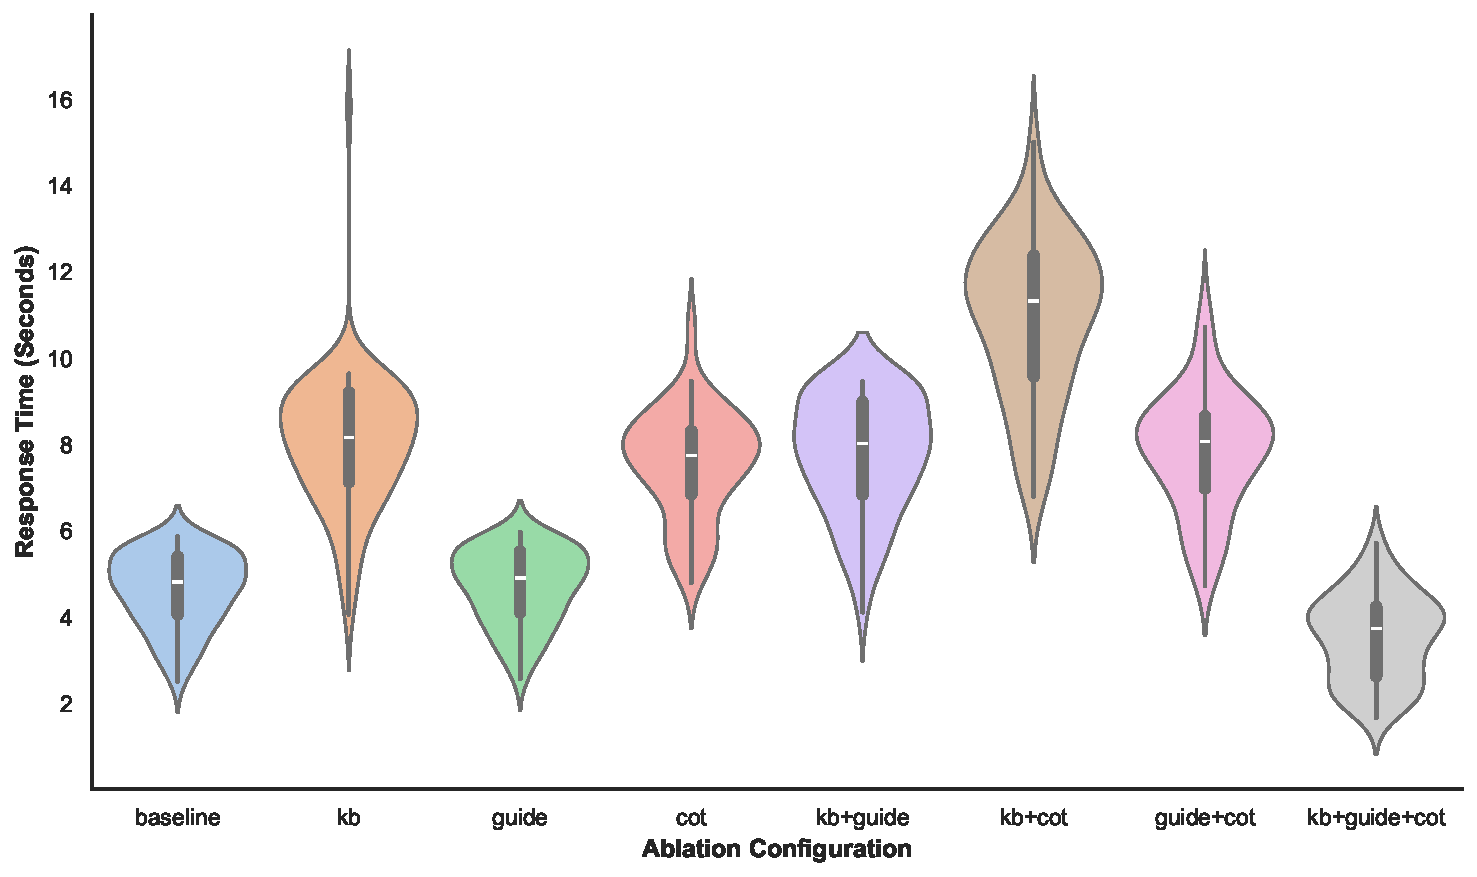
\includegraphics[width=0.9\textwidth]{time.pdf} % 后续插入时间分布图
\vspace{3cm} % 预留高度
\caption{Qwen3-VL-8B-Instruct-AWQ-4bit 在不同配置下响应时间的小提琴图分布}
\label{fig:violin}
\end{figure}

\subsubsection{模型横向对比与性能分析}
在确定了最优的提示词策略（KB+Guide+CoT）后，我们横向对比了多款模型的综合性能（包含准确率与平均推理时间），结果如表\ref{tab:model_cmp}所示。

\begin{table}[h]
\centering
\caption{各模型在最优策略 (KB+Guide+CoT) 下的综合性能对比}
\label{tab:model_cmp}
\begin{tabular}{lcccc}
\toprule
\textbf{模型名称} & \textbf{正确率 (\%)} & \textbf{拒识率 (\%)} & \textbf{误识率 (\%)} & \textbf{平均耗时 (s)} \\
\midrule
Qwen3-VL-4B-Instruct & 88 & 0 & 12 & 4.70 \\
Qwen2.5-VL-7B-Instruct-AWQ & 75 & 8 & 18 & 17.18 \\
Qwen3-VL-8B-Instruct & 99 & 1 & 0 & 20.55 \\
Qwen3-VL-8B-Instruct-AWQ-4bit & \textbf{100} & \textbf{0} & \textbf{0} & \textbf{3.54} \\
Qwen3-VL-32B-Instruct & 100 & 0 & 0 & 57.85 \\
\bottomrule
\end{tabular}
\end{table}

基于表\ref{tab:model_cmp}的测试数据，我们得出以下关键结论：
\begin{enumerate}
    \item \textbf{参数规模的权衡（8B为最佳甜点位）}：4B级别的小模型在面对曲面反光文本时能力显著不足，产生了高达12\%的误识率，这在医疗场景中是不可接受的；而32B超大模型虽然能完美实现100\%准确率，但单次推理耗时高达57.85秒，存在严重的算力浪费。相比之下，8B模型在能力上已完全能够保障高准确率与零误识。
    \item \textbf{量化技术的巨大工程收益}：对比Qwen3-VL-8B的原版与AWQ-4bit量化版，量化不仅没有导致精度折损（正确率保持在100\%），反而带来了极为显著的加速效果。平均响应时间从20.55秒显著下降至3.54秒，实现了近6倍的提速。
    \item \textbf{模型代际能力的飞跃（Qwen3 vs Qwen2.5）}：在相同的量化配置下，上一代Qwen2.5-VL-7B的正确率仅为75\%，而Qwen3-VL-8B达到了100\%。这印证了最新一代VLM在视觉特征提取与复杂指令遵循（尤其是约束规避指令）能力上的质变。
\end{enumerate}

综上所述，我们得出结论：在保证速度越快越好、正确率越高越好的双重目标下，\textbf{4-bit量化的8B模型（Qwen3-VL-8B-Instruct-AWQ-4bit）}是当前曲面药瓶识别任务的最优工程解。

\subsection{数据输入示例}
为了直观展示系统的输入形式，我们选取了代表性的药瓶旋转视频，将其连续帧截图并拼接展示，如图\ref{fig:frames}所示。由于均在高清工业相机下录制，多帧图像能够完整覆盖瓶身的不同视角，为大模型提供充足的上下文线索。

\begin{figure}[h]
\centering
% \includegraphics[width=1.0\textwidth]{frames_placeholder.pdf} % 后续插入多帧拼接图
\vspace{5cm} % 预留高度
\caption{药瓶多帧视频数据截取拼接示例。}
\label{fig:frames}
\end{figure}

\section{结论}
本文提出了一种基于视觉大语言模型（VLM）的曲面药瓶文本识别系统。该系统通过硬件采集药瓶多视角视频，结合自适应图像处理与多维度提示词工程（知识库+约束准则+思维链），成功攻克了曲面OCR在复杂反光与遮挡下的识别难题。通过对模型规模、代际和量化策略的深度对比实验，我们证明了8B级别的VLM在经过4-bit量化后，能够以极低的推理延迟（~3.5秒）实现100\%的准确率与极低的误识风险。本文为医疗包装识别及工业界替代高成本模板匹配方案，提供了一套高可靠、低成本且易于部署的全新范式。

尽管本系统在当前测试集上表现优异，但仍存在一定的局限性。例如，当药瓶标签遭受大面积物理撕毁、被严重污损覆盖导致有效文字信息彻底丢失，或者在完全无光的极端环境下，系统依然会面临视觉特征提取的挑战。在这种情况下，系统将高度依赖约束准则（拒识机制）输出“未知”，从而增加人工复核的成本。未来工作将探索引入多模态融合（如结合重量、外形轮廓等物理特征），以进一步提升极端工况下的自动化识别能力。

\begin{thebibliography}{99}
\bibitem{liu2019curved}
Liu, Y., Jin, L., Zhang, S., et al. (2019). Curved scene text detection via transverse and longitudinal sequence connection. \textit{Pattern Recognition}, 90, 337-345.

\bibitem{zhang2023printing}
Liu, Y., Li, J., et al. (2023). Printing Defect Detection Based on Scale-Adaptive Template Matching and Image Alignment. \textit{Sensors}, 23(9), 4414.

\bibitem{shi2023exploring}
Shi, Y., et al. (2023). Exploring OCR capabilities of GPT-4V(ision). \textit{arXiv preprint arXiv:2310.16809}.

\bibitem{qwen_vl}
Bai, S., et al. (2025). Qwen3-VL Technical Report. \textit{arXiv preprint arXiv:2511.21631}.

\bibitem{wang2024qwen2}
Wang, P., Bai, S., Tan, S., et al. (2024). Qwen2-VL: Enhancing Vision-Language Model's Perception of the World at Any Resolution. \textit{arXiv preprint arXiv:2409.12191}.

\end{thebibliography}

\end{document}
